\chapter{Projektformulering} \label{ch:projektformulering}
\section*{Version}
\begin{table}[h]
	\centering
	\begin{tabularx}{\textwidth - 2cm}{|l|l|l|X|}
	\hline
	Dato			& Version			& Initialer 		& Ændring										\\ \hline
	29. september 	& 1 				& Alle				& Første udkast. 								\\ \hline
	26. oktober		& 2 				& PKP, KT og JEP	& Mindre rettelser efter review					\\ \hline
	29.	oktober		& 3 				& PKP, KE 			& mindre rettelser efter vejledermøde			\\ \hline
	12.	november    & 4 				& KSN og HBJ		& Rettelser til usecases og PC protokol			\\ \hline
	13.	november    & 5 				& KSN       		& Rettelser til PC protokol						\\ \hline
	10.	december    & 6 				& PKP       		& Opdateret ordliste							\\ \hline
	\end{tabularx}
\end{table}

\section*{Indledning}
Følgende kapitel omfatter beskrivelse af opgaven samt definition af omfanget af projektet.
Ydermere er en ordforklaring beskrevet, som bedes konsulteres såfremt der er udtryk eller vendinger der ikke umiddelbart giver mening.

\clearpage

\section{Problemformulering} \label{sec:problemformulering}
Ifølge Niklas Alexander Chimirri, forsker inden for områder som barndom, psykologi og teknologi ved Roskilde Universitet, er leg en vigtig del af børns opvækst \cite{lib:RUC}.   
Det er essentielt for deres fremtid da det gør børnene sociale, robuste, kreative og ikke mindst nysgerrige. Med til at skabe rammerne for børns leg er legetøj, og i dagens Danmark er det vigtigt at børn har mulighed for at anvende den teknologi der er til rådighed. 
Dette bekræftes i en artikel der er udgivet på Roskilde Universitets hjemmeside i november 2014.
Han konkluderer at der er for stor forskel imellem den virkelighed børnene møder i, og uden for børnehaven ift. den teknologi der i dag er til rådighed. 

%---------------------------------------------------------------------------------------
%											PROJEKTBESKRIVELSE
%---------------------------------------------------------------------------------------

\section{Projektbeskrivelse} \label{sec:beskrivelse}


Projektet skal bidrage til eller i det mindste sætte fokus på, at det er vigtigt at børn har muligheden for at lege... og gerne med moderne teknologi. Derfor omhandler projektet design og implementering af en fjernstyret bil. Det skal ikke være en almindelig fjernstyret bil - den skal være intelligent og den får navnet ’’AU2’’. En skitse af bilen er vist på figur \ref{fig:rigbillede}.

Den intelligente del består af sensorer samt en kommunikationsenheder, som gør det muligt at styre bilen over et trådløst netværk. Brugeren har hermed mulighed for at navigere bilen ved at betragte en computerskærm, der viser et live-stream med video fra et kamera monteret på bilen. Er bilen inden for synsfeltet kan den selvfølgelig også styres ved at se direkte på den. For at undvige forhindringer på kørebanen, implementeres et anti-kollisionssystem bestående af afstandssensorer på bilen, placeret sådan at de kan detektere om bilen nærmer sig en forhindring. Således kan bilen selv kan standse eller undvige, hvis den nærmer sig en forhindring hastigt. Anti-kollisionssystemet har til formål at  forhindre en evt. kollision og derved beskadigelse af bilen eller dens omgivelser.

\begin{figure}[h]
\centering
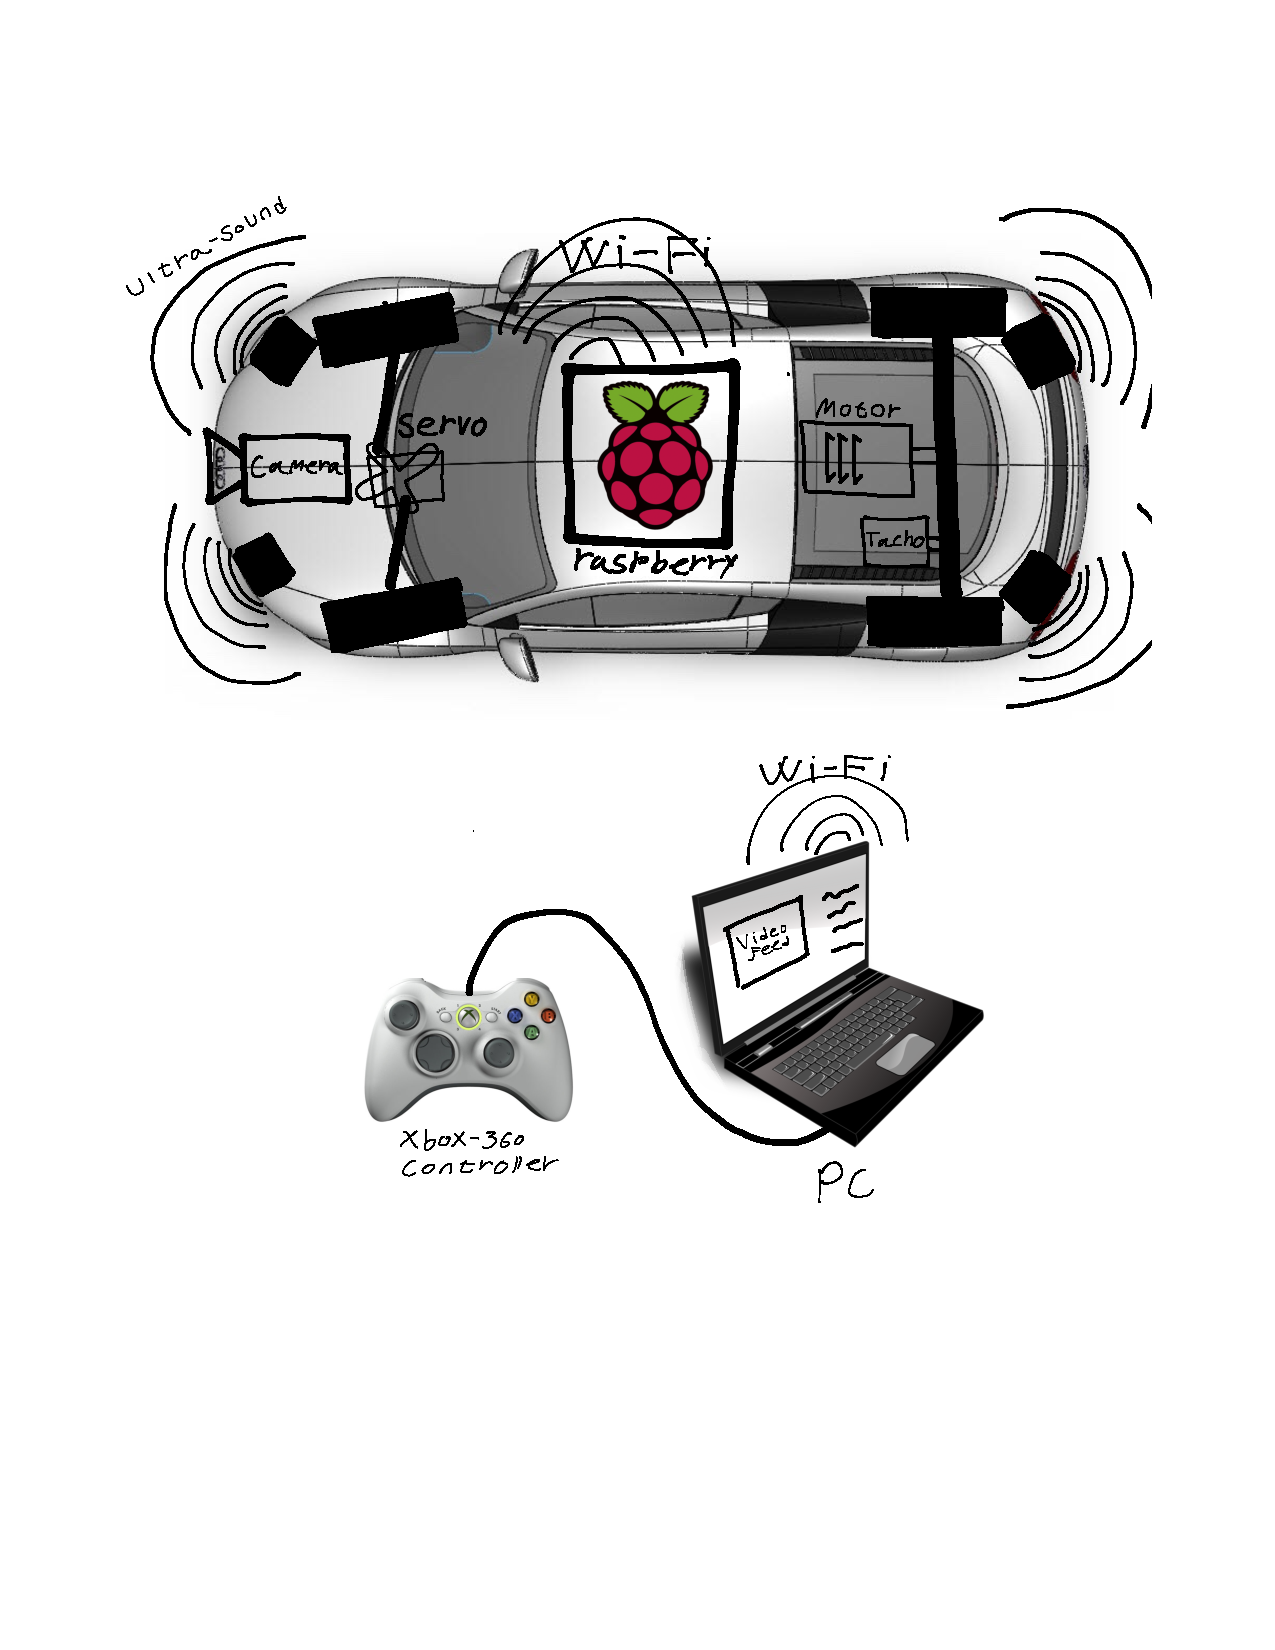
\includegraphics[width=\textwidth - 7.38 cm]{../fig/billeder/rigbillede}
\caption{Rigt billede af systemet i sin helhed}
\label{fig:rigbillede}
\end{figure}

\clearpage

%---------------------------------------------------------------------------------------
%											ORDBESKRIVELSE
%---------------------------------------------------------------------------------------

%==================== Ordforklaring ====================

\section{Ordforklaring}

\subsubsection{System}
Det totale system, indeholdende både bil, software på PC og netværkskommunikation mellem Bil og PC. 

\subsubsection{Human Interface Device (HID)}
En måde at kommunikere med en computer fx et tastatur, eller for dette projekts tilfælde, en XBOX360 controller.

\begin{itemize}
	\item Right Trigger (RT) - ??
	\item Left Trigger (LT) - ??
	\item Flere knapper her.
	%TODO list alle knapper på XBOX controller
\end{itemize}

\subsubsection{Hovedmenu}
Hovedmenuen i software på PC, indeholder menupunkter, som brugeren kan navigere efter behov.

\subsubsection{Bil}
Køretøjet samt controller som udfører alle relevante opgaver for bilen. Alt kommunikation med PC, foregår gennem denne.

\subsubsection{Wi-Fi}
Trådløst netværk af specifikationerne ''IEEE 802.11'', som Bil og PC kommunikerer over.

\subsubsection{Anti-kollitionssystem (AKS)}
Et system på bilen bestående af fire ultralydssensorer, som er i stand til at forhindre en kollision ved at overtage styringen fra Bruger i tilfælde af en kollisionskurs. Der gøres forskel mellem "Aktiver AKS" og "Tænd/Sluk AKS".

\begin{itemize}
	\item Tænd/Sluk bruges i forbindelse med at slå AKS fra eller til, således bilen ikke vil undgå en kollision hvis slukket, men vil undgå en kollsion hvis tændt. 
	\item AKS aktiveres ifm. at bilen er på vej til at kollidere med en forhindring, hvorefter bilen vil forhindre en kollision (AKS tændt) eller ej (AKS slukket).
\end{itemize}

\subsubsection{Ultralydssensorer}
Ultralydssensorerne benævnes herefter som hhv. Front Left (FL), Front Right (FR), Rear Left (RL) og Rear Right (RR). 

\clearpage 					 